\documentclass[12pt]{article}
\usepackage[utf8]{inputenc}
\usepackage[english]{babel}
\usepackage{amsmath, amsthm, amssymb, amsfonts}
\usepackage[top = 3in, left = 1in, right = 1in]{geometry}
\usepackage{hyperref, cleveref}
\hypersetup{
	colorlinks=true,
	linkcolor=blue,
	filecolor=magenta,      
	urlcolor=blue,
}
\usepackage{tcolorbox}
\usepackage{bm}


% FOR TIKZ
\usepackage{tikz}
\usetikzlibrary{arrows,arrows.meta, shapes.geometric}




% DEFINE NEW COMMANDS AND ENVIRONMENTS
\newcommand{\R}{\mathbb{R}}
\newcommand{\C}{\mathbb{C}}
\newcommand{\N}{\mathbb{N}}
\newcommand{\Q}{\mathbb{Q}}
\newcommand{\Z}{\mathbb{Z}}
\newcommand{\E}{\mathbb{E}}
\newcommand{\Var}{\mathbb{V}\text{ar}}
\newcommand{\Cinf}{\overline{\mathbb{C}}}
\newcommand{\res}{\text{Res}}


\newcommand{\HRule}{\rule{\linewidth}{0.5mm}} % Defines a new command for the horizontal lines, change thickness here


% DEFINE A PROBLEM Environment
\theoremstyle{definition}
\newtheorem*{prb}{Problem}
\newenvironment{problem}{
\begin{tcolorbox}[colback=blue!5!white,colframe=blue!75!black, parbox = true] \begin{prb}  }{\end{prb}\end{tcolorbox} }
\newenvironment{answer}{\textit{Solution: }\quad }{ \hfill $\blacksquare$}
\newtheorem{claim}{Claim}


\numberwithin{equation}{section}


\begin{document}


% TITLE PAGE
%%%%%%%%%%%%%%%%%%%%%%%%%%%%%%%%%%%%%%%%%%%%%%%%%%%%%%
\begin{titlepage}
    
\centering
\textsc{\LARGE Indian Statistical Institute, Kolkata}\\[1.5cm] % Name of your university/college
\textsc{\Large Metric Topology and Complex Analysis}\\[0.5cm] % Major heading such as course name
\textsc{\large Final examination: Second Semester 2019-2020}\\[0.5cm] % Minor heading such as course title

\HRule \\[0.4cm]
\large \textbf{Subhrajyoty Roy}\\
\large \textbf{Roll:  MB1911}\\
\HRule \\[1.5cm]
\normalsize \today

\end{titlepage}


\tableofcontents
\clearpage


% CONTENT FROM HERE
%%%%%%%%%%%%%%%%%%%%%%%%%%%%%%%%%%%%%%%%%%%%%%%%%%
\newgeometry{margin = 1in}

\section{Problem 1}

\begin{problem}
	Where does the function $f(z) = z \Re(z) + \bar{z} \Im(z) + \bar{z}$ have a complex derivative? Find the derivative wherever it exists. 

	\textbf{Notation:} $\Re(z), \Im(z)$ are respectively the real and imaginary parts of $z$. 
\end{problem}

\begin{answer}
	We start by considering $z = (x + iy)$, where $x, y\in \R$. Then,
	
	\begin{align*}
		f(z)
		& = z \Re(z) + \bar{z} \Im(z) + \bar{z}\\
		& = (x + iy) x + (x - iy)y + (x - iy)\\
		& = x^2 + ixy + xy - iy^2 + x - iy\\
		& = (x^2 + xy + x) + i(xy - y^2 - y)\\
		& = u(x, y) + i v(x, y)
	\end{align*}

	where $u$ and $v$ are the real quantities they are replacing. Now, if $f$ is analytic at $z = z_0 = (x_0 + i y_0)$, it must satisfy the Cacuhy-Riemann equations at that point, i.e. we must have,

	$$
	\dfrac{\partial u}{\partial x}(z_0) = \dfrac{\partial v}{\partial y}(z_0) \qquad \text{ and } \qquad \dfrac{\partial u}{\partial y}(z_0) = -\dfrac{\partial v}{\partial x}(z_0)
	$$

	However,

	\begin{align*}
		\dfrac{\partial u}{\partial x}(z_0) & = (2x_0 + y_0 + 1) \\
		\dfrac{\partial v}{\partial y}(z_0) & = (x_0 - 2y_0 - 1)\\
		\dfrac{\partial u}{\partial y}(z_0) & = x_0 \\
		\dfrac{\partial v}{\partial x}(z_0) & = y_0\\
	\end{align*}

	Thus, at the point $z_0$ where $f$ is analytic, we must have $(2x_0 + y_0 + 1) = (x_0 - 2y_0 - 1)$, i.e. $x_0 + 3y_0 = (-2)$ and $x_0 = (-y_0)$. These two equations solves to yield the solution $x_0 = 1$ and $y_0 = (-1)$, i.e. $z_0 = (1 - i)$.

	Therefore, it shows that $f(z)$ is not complex differentiable at any point except possibly $z = (1 - i)$. Now, we try to see if the derivative exists at this particular point.

	Firstly note that, 

	$$
	f(1-i) = (1-i)\times 1 + (1+i)\times (-1) + (1+i) = (1-i)
	$$

	Let, $h = h_1 + i h_2$ and consider the following:

	\begin{align*}
		& \dfrac{f((1-i)+ h) - f(1-i)}{h}\\
		= \quad & \dfrac{f( (1+h_1) + i(h_2 - 1) ) - (1 - i)}{h}\\
		= \quad & \dfrac{ ((1+h_1)+i(h_2 - 1))(1+h_1) + ((1+h_1)-i(h_2 - 1))(h_2 - 1) + ((1+h_1)-i(h_2 - 1)) - (1-i)  }{h}\\
		= \quad & \dfrac{ ((1+h_1)+i(h_2 - 1))(1+h_1) + ((1+h_1)-i(h_2 - 1))h_2 - (1-i)  }{h}\\
		= \quad & \dfrac{ \left[(1+h_1)(1 + h_1 + h_2) - 1\right] + i \left[ (h_2 - 1)(1 + h_1 - h_2) + 1 \right] }{h}\\
		= \quad & \dfrac{\left[h_1^2 + h_1h_2 + 2h_1 + h_2\right] + i \left[ h_2h_1 - h_2^2 -h_1 + 2h_2 \right]}{h}\\
		= \quad & \dfrac{2(h_1 + ih_2) + h_1(h_1 + ih_2) - i(h_1 + ih_2) + (h_1 h_2 - ih_2^2)}{h}\\
		= \quad & (2+h_1 - i) + \dfrac{(h_1 h_2 - ih_2^2)}{h}\\
	\end{align*}

	So now, we consider,

	\begin{align*}
		\left\vert \dfrac{f((1-i)+ h) - f(1-i)}{h} - (2-i) \right\vert
		& = \left\vert h_1 + \dfrac{(h_1 h_2 - ih_2^2)}{h} \right\vert\\
		& \leq \vert h_1 \vert + \dfrac{\vert h_1h_2 - ih_2^2 \vert}{ \vert h \vert} \qquad \text{, by triangle inequality}\\
		& = \vert h_1 \vert + \dfrac{\vert h_2 \vert \vert h_1 - ih_2 \vert}{\vert h \vert}\\
		& = \vert h_1 \vert + \dfrac{\vert h_2 \vert \vert \bar{h}\vert}{\vert h \vert}\\
		& = \vert h_1 \vert + \vert h_2 \vert \qquad \text{, since } \vert \bar{z} \vert = \vert z \vert\\
		& \leq 2 \vert h \vert\\
		& \rightarrow 0 \quad \text{, as } \vert h \vert \rightarrow 0
	\end{align*}

	Therefore, by definition of limit and complex derivative,

	$$
	f'(1-i) = \lim_{\vert h \vert \rightarrow 0} \dfrac{f((1-i)+ h) - f(1-i)}{h} = (2-i)
	$$

	Thus, $f(z)$ has a complex derivative only at the point $z = (1-i)$ and the derivative at that point is $f'(1-i) = (2-i)$.


\end{answer}

\pagebreak

\section{Problem 2}
\begin{problem}
	\begin{enumerate}
		\item[(i)] Show that a M\"{o}bius transformation (except identity transformation) has $0$ and $\infty$ as its only fixed points iff it is
		a dilation.
		\item[(ii)] Find the image of the set $\{z : |z| < 1\} \cap \{z : |z - 1| < 1\}$ under the map $Tz = \dfrac{z-1}{z+1}$.
	\end{enumerate}
\end{problem}

\begin{answer}
	\begin{enumerate}
		\item[(i)]
		
		\textbf{If part:} Let us assume the M\"{o}bius transformation is a dilation, namely $S(z) = az$ for some $a \neq 0, a\in \C$\footnote{Here, $a$ can be a complex number, in that case, the rotation becomes a special case of dilation.}.

		Then, $S(z) = z$ implies, $az = z$. Clearly, as $a \neq 0$, and $a \neq 1$ (because of the exemption on identity transformation). Now, it is easy to see that $0$ and $\infty$ are indeed two fixed points of the transformation, as $S(0) = a\times 0 = 0$ and $S(\infty) = a \times \infty = \infty$, as $a \neq 0$. Finally, to show that these are the only fixed point, assume for some $z \in \C$ with $0 < \vert z \vert < \infty$, it is a fixed point of the transformation. Then, $S(z) = z$ holds. That is, $az = z$, and then multiplying $z^{-1}$ to both sides (which exists as $0 < \vert z \vert < \infty$), we obtain $a = 1$, in contradiction to the assumption that identity transformation is exempted.

		\textbf{Only if Part:} In this case, we consider a general M\"{o}bius transformation as a follows:

		$$
		S(z) = \dfrac{az + b}{cz + d} \qquad \text{ with } (ad - bc) \neq 0
		$$

		Now, it is given that the only fixed points of the above transformation is $0$ and $\infty$. Thus we have,

		$$
		S(0) = 0 \Rightarrow \dfrac{b}{d} = 0 \Rightarrow b = 0
		$$

		and 

		\begin{align*}
			S(\infty) = \infty \Rightarrow \lim_{z \rightarrow \infty} \dfrac{1}{S(z)} = 0
			\Rightarrow & \lim_{z \rightarrow \infty} \dfrac{cz+d}{az + b} = 0 \\
			\Rightarrow & \lim_{z \rightarrow \infty} \dfrac{c+(b/z)}{a + (d/z)} = 0 \Rightarrow \dfrac{c}{a} = 0
			\Rightarrow c = 0			
		\end{align*}

		Thus, we have $S(z) = \dfrac{a}{d}z$. Now, as $(ad - bc)\neq 0$, this implies that $d \neq 0$ and hence the transformation is well defined. Also, $a \neq 0$, and thus $(a/d) \neq 0$. Taking $\lambda = (a/d)$, we obtain $S(z) = \lambda z$, where $\lambda \in \C$ and $\lambda \neq 0$, which is a dilation. 

		\item[(ii)] Let, $\Cinf = \C \cup \{ \infty \}$. To find the image of the set $\{ z : \vert z \vert < 1 \} \cap \{ z : \vert z - 1\vert < 1 \}$ under the M\"{o}bius transformation mentioned in the question, 
		we employ the following result.

		\begin{center}
			\textit{A M\"{o}bius transformation maps a circle in $\Cinf$ to a circle in $\Cinf$.}
		\end{center}

		So, we conisder the two circles $A = \{ z : \vert z \vert < 1\}$ and $B = \{ z : \vert z - 1 \vert < 1 \}$. Let, $T(z) = \dfrac{(z - 1)}{(z + 1)}$, the given M\"{o}bius transformation.
		
		Let us first choose three points on the boundary circle $\partial A$, as $1, (-i)$ and $i$. Note that, 

		$$
		T(1) = 0 \quad \text{ and } \quad
		T(-i) = (-i) \quad \text{ and } \quad
		T(i) = i
		$$

		Clearly, image of $\partial A$ must be a circle in $\Cinf$, and these values must lie on that circle. Clearly, these outputs $0, (-i)$ and $i$ are actually collinear and lie on the imaginary axis of the argand plane. To find which side of the imaginary axis actually corresponds to the image of the inside disc of $A$, consider the origin which lies inside $A$ and $T(z) = (-1)$, thus image of $A$ under the transformation $T$ is basically $\{ z : \Re(z) < 0 \}$.

		In a similar way, we choose three points on the boundary circle $\partial B$, as $0, 2, (1+i)$. Then,

		$$
		T(0) = (-1) \quad \text{ and } \quad
		T(2) = \dfrac{1}{3} \quad \text{ and } \quad
		T(1+i) = \dfrac{(1 + 2i)}{5}
		$$

		Now, to find the unique circle passing through these 3 points, we consider the general equation of a circle $(x - a)^2 + (y-b)^2 = r^2$. Clearly, the points $(-1, 0), (1/3, 0)$ and $(1/5, 2/5)$ satisfy the equation. Hence, we have the following:

		\begin{align*}
			& (1 + a)^2 + b^2 = r^2\\
			& (1/3 - a)^2 + b^2 = r^2\\
			& (1/5 - a)^2 + (2/5 - b)^2 = r^2
		\end{align*}

		Solving for $a$, $b$ and $r$ yields, $a = (-1/3)$ and $b = 0$, and $r = 2/3$.  Therefore, the image of the circle $\partial B$ is given by the circle centered at $(-1/3)$ and radius $2/3$. To find whether the image of $B$ lies inside the circle, we consider a point $1 \in B$, and as $T(1) = 0$ lies inside the circle, we have the image of the disc $B$ as $\{ z : \vert z - 1/3 \vert < 2/3\}$. 

		Therefore, combining these all, we obtain that the image of $A \cap B$ under the map $T$ is given by;

		$$
		\{ z : \Re(z) < 0\} \cap \{ z : \vert z - 1/3 \vert < 2/3 \}
		$$

	\end{enumerate}
\end{answer}

\pagebreak

\section{Problem 3}
\begin{problem}
	$f : \Omega \rightarrow \C$ is an analytic function where $\Omega$ is an open connected set containing the closure of the unit disc $D = \{ z\in\C : |z| < 1\}$. Show that, if $f$ is real on the boundary of $D$, then $f$ must be constant.
\end{problem}

\begin{answer}
	
	Since, we need to prove that $f$ is constant, it is tempting to use Liouville's theorem in order to get our desired result. However, since $f$ is not given to be entire function, the theorem cannot be applied directly.

	With that in mind, we consider the following function:

	$$
	g(z) = \begin{cases}
		\overline{f(\overline{z})} & \text{ if } \vert z \vert \leq 1\\
		f(1/z) & \text{ if } \vert z \vert > 1
	\end{cases}
	$$

	Clearly, $g : \C \rightarrow \C$. Note that, for $z \in \partial D$, $\vert z \vert = 1$ and $\vert \overline{z} \vert = \vert (1/z) \vert$ and as $f$ takes only real value on the boundary $\partial D$,, it must be that $\overline{f(\overline{z})} = f(1/z)$ for all $z \in \partial D$.
	
	
	We shall show that $g$ is entire and bounded.

	\begin{enumerate}
		\item \textbf{Boundedness:} To show that $g$ is bounded, consider the closed unit disc $\{ z : \vert z \vert \leq 1 \}$, which being closed and bounded in $\R^2 \equiv \C$ is compact in $\R^2$, hence compact in $\Omega$. 
		
		Since, $f$ is known to be analytic in $\Omega$, it is continuous in $\Omega$, hence is bounded in the unit disc, i.e. there exists a real number $\infty > M > 0$ such that, $\vert f(z) \vert < M$ for all $\vert z \vert \leq 1$.

		Now, if $\vert z \vert \leq 1$, clearly;

		$$\vert \overline{f(\overline{z})} \vert = \vert f(\overline{z}) \vert < M$$
		
		as $\vert \overline{z} \vert \leq 1$.

		On the other hand, if $\vert z \vert > 1$, then $\vert (1/z) \vert \leq 1$, thus $\vert f(1/z) \vert < M$. Therefore, it follows that $g(z)$ is a bounded function for any $z \in \C$.

		\item \textbf{Analyticity: } To show that $g$ is analytic everywhere, we shall be using Morera's theorem. Let us consider a triangle $T$ such that the triangle and the region enclosed by it lies within the extended domain $\C$. 
		
		Let us consider three subcases:

		\begin{enumerate}
			\item If the triangle $T$ lies entirely within the unit disc $D$, then 
			
			$$\displaystyle\int_T g(z) dz = \displaystyle\int_T \overline{f(\overline{z})} dz$$
			
			To show that it is equal to $0$, all we need to show is the function $\overline{f(\overline{z})}$ is analytic within the disc, hence an application of Cacuhy's theorem on the closed curve $T$ would yield the result.

			To see why, $\overline{f(\overline{z})}$ is analytic at some point $z_0 \in D$, note that, since $z_0 \in D$, $\overline{z_0} \in D$, and thus $f$ is analytic at $\overline{z_0}$. Considering a power series representation of $f$ at the neighbourhood of $\overline{z_0}$, we get;

			$$
			f(z) = \sum_{n = 0}^{\infty} a_n (z - \overline{z_0})^n
			$$

			for $z$ being in some neighbourhood around $\overline{z_0}$. 

			Thus,

			$$
			\overline{f(\overline{z})} = \overline{\sum_{n = 0}^{\infty} a_n (\overline{z} - \overline{z_0})^n} = \sum_{n = 0}^{\infty} \overline{a_n (\overline{z} - \overline{z_0})^n} = \sum_{n = 0}^{\infty} \overline{a_n} (z - z_0)^n
			$$

			which gives a power series representation of $\overline{f(\overline{z})}$ around the point $z_0 \in D$. Since, $\vert a_n \vert = \vert \overline{a_n} \vert$, the radius of convergence for both of these power series are same. This shows that $\overline{f(\overline{z})}$ is analytic, and hence $\int_T g(z)dz = 0$ if $T$ lies completely in $D$.

			\item If the triangle $T$ lies completely outside the unit disc $D$, then by similar logic,
			
			$$
			\int_T g(z)dz = \int_T f(1/z)dz = 0
			$$

			where the last equality follows again from Cauchy's theorem and analyticity of $f(1/z)$ for any $\vert z \vert > 1$, which follows as $f(z)$ is analytic for any $\vert z \vert < 1$.

			\item  Finally, if the triangle $T$ lies partly inside the unit disc $D$, and lies partly outside the disc, we divide the triangle into two parts, $(T \cap D)$ and $(T \cap D^c)$, as indicated in the figure.
			
			\begin{figure}[h]
				\centering
				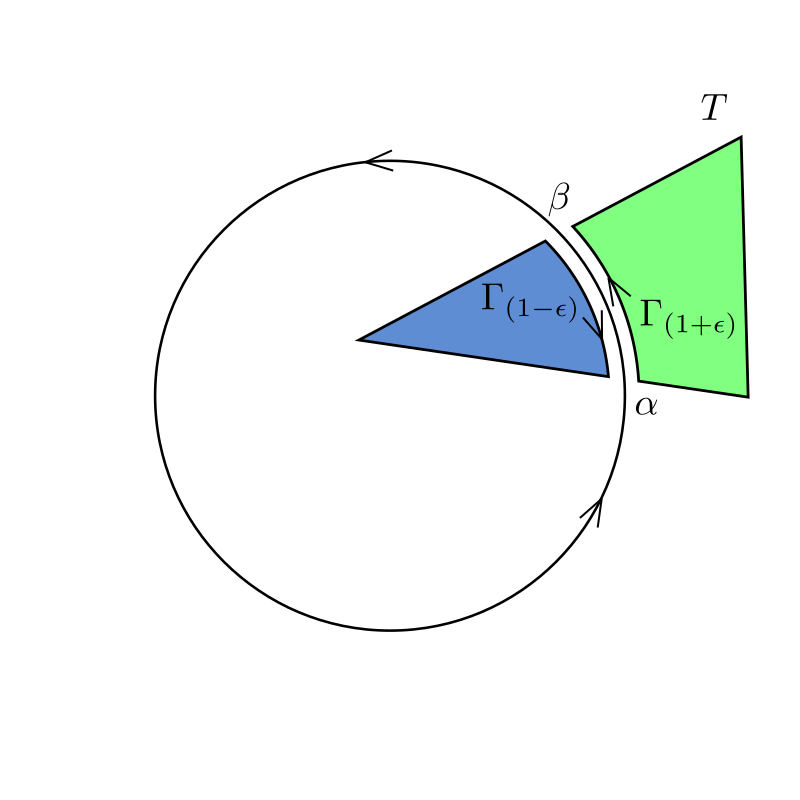
\includegraphics[width = 0.5\linewidth]{circle-arc.png}
			\end{figure}

			The blue region in the above figure is $\{ z : z\in T , \vert z \vert \leq (1- \epsilon) \}$ and the green region in $\{ z : z \in T, \vert z \vert \geq (1 + \epsilon) \}$, where $\epsilon > 0$ is chosen by us.

			Note that, again by application of Cauchy's theorem, the integral of $g(z)$ over the boundary of blue region with a positive orientation is $0$, since $g$ is analytic everywhere within that blue region. Similarly, the integral of $g(z)$ over the boundary of green region with a negative orientation is also $0$ by Cauchy's theorem, since $g$ is analytic everywhere within that green region. We can simply let $\epsilon \rightarrow 0$ and obtain the integral $\int_T g(z)dz$ as long as the integral over the arc $\Gamma_{(1 -\epsilon)}$ and $\Gamma_{(1 + \epsilon)}$ cancels out.

			To see this, consider the parametrization $\Gamma_r(\theta) = r e^{i\theta}$ for $r = (1-\epsilon)$ or $(1 + \epsilon)$. Then,

			\begin{align*}
				& \left\vert \int_{\Gamma_{(1 - \epsilon)}} g(z)dz + \int_{\Gamma_{(1 + \epsilon)}} g(z)dz \right\vert\\
				= \quad & \left\vert \int_{\Gamma_{(1 - \epsilon)}} \overline{f(\overline{z})} dz + \int_{\Gamma_{(1 + \epsilon)}} f(1/z)dz \right\vert \\
				= \quad & \left\vert \int_{\beta}^{\alpha} \overline{f(\overline{(1-\epsilon)e^{i\theta}} )} (1-\epsilon)i e^{i\theta}d\theta + \int_{\alpha}^{\beta} f\left( \dfrac{1}{(1+\epsilon) e^{i\theta}}\right)(1 + \epsilon)ie^{i\theta}d\theta \right\vert\\
				\leq \quad & \int_{\alpha}^{\beta} \left\vert f\left( \dfrac{e^{-i\theta}}{(1 + \epsilon)} \right) (1+\epsilon) - \overline{f((1-\epsilon) e^{-i\theta})}(1 - \epsilon) \right\vert \vert i e^{i\theta} \vert d\theta\\
				= \quad & \int_{\alpha}^{\beta} \left\vert f\left( \dfrac{e^{-i\theta}}{(1 + \epsilon)} \right) (1+\epsilon) - \overline{f((1-\epsilon) e^{-i\theta})}(1 - \epsilon) \right\vert d\theta\\
				= \quad & \int_{\alpha}^{\beta} \left\vert (1+\epsilon)f\left( \dfrac{e^{-i\theta}}{(1 + \epsilon)} \right) - (1 + \epsilon)f(e^{-i\theta}) \right. \\
				& \qquad \qquad \left. + (1 - \epsilon) \overline{f(e^{-i\theta})} - (1 - \epsilon) \overline{f((1-\epsilon) e^{-i\theta})} + 2\epsilon f(e^{-i\theta}) \right\vert d\theta\\
				& \qquad \qquad  \text{, since } e^{-i\theta} \in \partial D \Rightarrow f(e^{-i\theta}) \in \R\\
				& \leq \int_{\alpha}^{\beta} (1 + \epsilon)\left\vert f\left( \dfrac{e^{-i\theta}}{(1 + \epsilon)} \right) - f(e^{-i\theta}) \right\vert \\
				& \qquad \qquad \qquad + (1-\epsilon)\left\vert f(e^{-i\theta}) - f((1-\epsilon)e^{-i\theta}) \right\vert
				+ 2\epsilon \vert f(e^{-i\theta}) \vert d\theta\\
			\end{align*}

			Now, the applying Mean Value Theorem, for some $\xi$ with $(1 - \epsilon) \leq \vert \xi \vert \leq 1$ and $\eta$ with $1 \leq \vert \eta \vert \leq (1 + \epsilon)$, and applying that $\vert e^{-i\theta} \vert = 1$,

			$$
			\left\vert f\left( \dfrac{e^{-i\theta}}{(1 + \epsilon)} \right) - f(e^{-i\theta}) \right\vert \leq \left\vert \dfrac{\partial f}{\partial r}(\xi) \left[\dfrac{e^{-i\theta}}{(1 + \epsilon)} - e^{-i\theta}\right] \right\vert = \left\vert \dfrac{\partial f}{\partial r}(\xi)\right\vert \dfrac{\epsilon}{(1 + \epsilon)}
			$$

			and 

			$$
			\vert f(e^{-i\theta}) - f((1-\epsilon)e^{-i\theta}) \vert \leq \left\vert \dfrac{\partial f}{\partial r}(\eta)\right\vert \vert e^{-i\theta} \epsilon \vert = \epsilon \left\vert \dfrac{\partial f}{\partial r}(\eta)\right\vert
			$$

			where $\dfrac{\partial f}{\partial r}$ denotes the partial derivative of $f$ with respect to the radius (Think of polar coordinate). However, since $f$ is analytic, it follows that these partial derivatives are continuous, and since $\eta$ and $\xi$ lies within a compact set (the ring with inner radius $(1 - \epsilon)$ and outer radius $(1 + \epsilon)$), these are bounded, say by some $B > 0$.

			Thus, combining everything,

			\begin{align*}
				& \left\vert \int_{\Gamma_{(1 - \epsilon)}} g(z)dz + \int_{\Gamma_{(1 + \epsilon)}} g(z)dz \right\vert\\
				\leq \quad & \int_{\alpha}^{\beta} \left[ \epsilon \left\vert \dfrac{\partial f}{\partial r}(\xi) \right\vert + \epsilon(1 - \epsilon) \left\vert \dfrac{\partial f}{\partial r}(\eta) \right\vert + 2\epsilon \vert f(e^{-i\theta}) \vert \right]d\theta\\
				< \quad & \epsilon (\beta - \alpha) (B + B + 2M) \rightarrow 0
			\end{align*}

			This means, the integral over those arcs with cancel each other, hence $\int_T g(z)dz = 0$ for any triangle $T$ which lies partially in the disc $D$ and lies partially outside it.

			Thus, for any triangle $T$, $\int_T g(z)dz = 0$. Therefore, using Morera's theorem, it follows $g$ is analytic everywhere in the complex plane.
		\end{enumerate}

		Thus, $g$ is entire and bounded function, by application of Liouville's theorem, it follows that $g(z)$ is constant. Say, $g(z) = c$ for all $z \in \C$. Now, this means, $\overline{f(\overline{z})} = c$, thus $f(\overline{z}) = \overline{c}$ for any $z$ with $\vert z \vert \leq 1$. Since then $\vert \overline{z} \vert \leq 1$, it follows $f$ is constant within the closed disc $\overline{D}$. 

		Since, $f(z)$ is constant in $\overline{D}$, $f'(z) = 0$ for any $z \in \overline{D}$. Also, as $f$ is analytic in $\Omega$, and $f'$ is also analytic in $\Omega$. Clearly, it follows that there is a sequence of zeros of $f'$ which has a limit point in $\Omega$. As $\Omega$ is connected open set, it follows $f'\equiv 0$\footnote{\textbf{Statement of the theorem:} Suppose, $f$ is analytic on a connected open set $\Omega$ and the zeroes of $f$ are a sequence of distinct points having a limit point in $\Omega$. Then $f$ is identically zero.}, thus $f(z)$ is constant for any $z \in \Omega$.

		This completes the proof.
	\end{enumerate}





\end{answer}


\pagebreak

\section{Problem 4}
\begin{problem}
	Evaluate the following integrals using residue formula.
	\begin{enumerate}
		\item[(i)] $\int_{|z| = 2} \dfrac{e^z}{\cos z}dz$
		\item[(ii)] $\int_{0}^{\pi} \dfrac{1}{5 + 3 \cos \theta} d\theta$ 
	\end{enumerate}
\end{problem}

\begin{answer}
	\begin{enumerate}
		\item[(i)] Consider the function $f(z) = \dfrac{e^z}{\cos z}$. Note that, as a function from $\C$ to $\C$, it is analytic everywhere except the points where $\cos z =0$, i.e. except the points $z = 2n\pi + \dfrac{\pi}{2}$ for some $n \in \Z$. 
		 
		Since, we want to find the integral over the circle $\vert z \vert = 2$, we need to look for poles within the disc $D$ of radius $2$ centered at the origin. Note that, there are only $2$ simple poles of $f(z)$ within $D$, namely at $z = \pi/2$ and $z = -\pi/2$.
		
		Therefore, by an application to Residue formula, we obtain;

		$$
		\int_{\vert z \vert = 2} \dfrac{e^z}{\cos z} dz = 2\pi i\left[\res_{z = \pi/2}(f) + \res_{z = -\pi/2}(f)\right]
		$$

		Now, since $z = \pi/2$ is a simple pole of $f$,

		\begin{align*}
			\res_{z = \pi/2}(f)
			& = \lim_{z \rightarrow \pi/2} \left( z - \dfrac{\pi}{2}\right) f(z)\\
			& = \lim_{z \rightarrow \pi/2} \left( z - \dfrac{\pi}{2}\right) \dfrac{e^z}{\cos z}\\
			& = \lim_{z \rightarrow \pi/2} e^z \times \lim_{z \rightarrow \pi/2} \dfrac{(z - \pi/2)}{\cos z}\\
			& = -e^{\pi/2} \qquad \text{, since } \dfrac{\cos z}{(z - \pi/2)} \rightarrow (-1) \text{ as } z \rightarrow \frac{\pi}{2}
		\end{align*}

		In a similar way, for the simple pole $z = -\pi/2$, 

		\begin{align*}
			\res_{z = -\pi/2}(f)
			& = \lim_{z \rightarrow -\pi/2} \left( z + \dfrac{\pi}{2}\right) f(z)\\
			& = \lim_{z \rightarrow -\pi/2} \left( z + \dfrac{\pi}{2}\right) \dfrac{e^z}{\cos z}\\
			& = \lim_{z \rightarrow -\pi/2} e^z \times \lim_{z \rightarrow -\pi/2} \dfrac{(z + \pi/2)}{\cos z}\\
			& = e^{-\pi/2} \qquad \text{, since } \dfrac{\cos z}{(z + \pi/2)} \rightarrow 1 \text{ as } z \rightarrow -\frac{\pi}{2}
		\end{align*}

		Therefore,

		$$
		\int_{\vert z \vert = 2} \dfrac{e^z}{\cos z} dz = 2\pi i \left[ e^{-\pi/2} - e^{\pi/ 2} \right]
		$$
		

		\item[(ii)] To compute the real integral using residue formula, we try to convert this into a complex integration along curves using some kind of parametrization. 
		
		Let us take, $z = \gamma(\theta) = e^{i\theta}$ as our parametrization. Then, $\gamma'(\theta) = i e^{i\theta} = iz$. Also, as $\theta$ goes from $0$ to $2\pi$, the parametrization $z$ travels along the unit circle centered at origin in a positive orientation.

		Now, note that the integral can be written as;

		\begin{align*}
			\int_{0}^{\pi} \dfrac{1}{5 + 3\cos \theta} d\theta
			& = \dfrac{1}{2} \left[ \int_{0}^{2\pi} \dfrac{1}{5 + 3 \cos \theta} d\theta\right] \qquad \text{, since } \dfrac{1}{5 + 3 \cos \theta} = \dfrac{1}{5 + 3 \cos (2\pi - \theta)}\\
			& = \dfrac{1}{2} \int_{0}^{2\pi} \dfrac{ie^{i\theta}}{(5 + 3 \cos \theta)ie^{i\theta}}d\theta\\
			& = \dfrac{1}{2} \int_{ \vert z \vert = 1} \dfrac{1}{\left(5 + 3 \dfrac{(z + z^{-1})}{2}\right) iz} dz\\
			& \qquad \qquad \text{by the parametrization and as } \cos \theta = \dfrac{e^{i\theta} + e^{-i\theta}}{2} = \dfrac{(z + z^{-1})}{2}\\
			& \\
			& = \dfrac{1}{2i} \int_{\vert z \vert = 1} \dfrac{2}{3z^2 + 10z + 3} dz\\
			& = \dfrac{1}{i} \int_{\vert z \vert = 1} \dfrac{1}{(3z + 1)(z + 3)}dz
		\end{align*}

		Now, consider the function $f(z) = \dfrac{1}{(3z + 1)(z+3)}$, which has two simple poles at $z = (-1/3)$ and $z = (-3)$, and is analytic everywhere else. However, as we are integrating over the unit circle centered at origin, only the pole $z = (-1/3)$ resides within the unit disc centered at origin. Thus, by an application of Residue formula, it follows that;

		$$
		\int_{\vert z \vert = 1} \dfrac{1}{(3z + 1)(z + 3)} = 2\pi i\res_{z = (-1/3)}(f)
		$$

		Since, $z = (-1/3)$ is a simple pole, we have,

		\begin{align*}
			\res_{z = (-1/3)}(f)
			& = \lim_{z \rightarrow (-1/3)} \left( z + \dfrac{1}{3} \right)f(z)\\
			& = \lim_{z \rightarrow (-1/3)} \dfrac{(3z + 1)}{3} \times \dfrac{1}{(3z + 1)(z+3)}\\
			& = \lim_{z \rightarrow (-1/3)} \dfrac{1}{3(z+3)}\\
			& = \dfrac{1}{8}
		\end{align*}

		Therefore,

		$$
		\int_{0}^{\pi} \dfrac{1}{5 + 3\cos \theta} d\theta = \dfrac{1}{i} 2\pi i \times \res_{z = (-1/3)}(f) = \dfrac{\pi}{4}
		$$

	\end{enumerate}
\end{answer}

\pagebreak

\section{Problem 5}
\begin{problem}
	Let $f$ be an analytic function in the region $\{ z : |z| > 1\}$ and suppose that $\lim_{z \rightarrow \infty} f(z) = 0$. Show that if $|z| > 2$, then 

	$$
	\dfrac{1}{2\pi i} \int_{|\xi| = 2} \dfrac{f(\xi)}{(\xi - z)}d\xi = -f(z)
	$$
\end{problem}


\begin{answer}
	Consider the following function, $g : \{ z : \vert z \vert < 1 \} \rightarrow \C$;

	$$
	g(z) = \begin{cases}
		f(1/z) & \text{ if } 1 > \vert z \vert > 0\\
		0 & \text{ if } z = 0
	\end{cases}
	$$

	Note that, since the function $f$ is analytic everywhere in $\{ z : \vert z \vert > 1 \}$, $g$ is analytic everywhere in $\{ z : \vert z \vert < 1\}$ except possibly at the point $z = 0$, the origin.

	Clearly, $g$ possibly has an isolated singularity at $z = 0$. Thus, we shall try to inspect which type of singularity it is. Note that, $\lim_{z \rightarrow 0} z g(z) = \lim_{z \rightarrow 0} z f(1/z) = 0$, as $\lim_{z \rightarrow \infty} f(z) = 0$, and thus $f(1/z)$ is bounded as $z \rightarrow 0$. Hence, it follows that $z = 0$ is a removable singularity of this function $g$. Therefore, there exists an extension of $g$, namely $h$, which agrees with $g$ at all points in $\{ z : \vert z \vert < 1\}$, except possibly at the origin. However, since $h$ is analytic everywhere inside the unit disc, it is continuous also. Hence,

	$$
	h(0) = \lim_{z \rightarrow 0}h(z) = \lim_{z \rightarrow 0}g(z) = \lim_{z \rightarrow 0} f(1/z) = \lim_{z \rightarrow \infty} f(z) = 0 = g(0)
	$$

	Thus, $g \equiv h$ at all points inside the unit disc, and hence $g$ is analytic inside the unit disc.

	Now, let $z\in \C$ be such that $\vert z \vert > 2$. Also, let $D$ denote the disc $\{ z : \vert z \vert = 1/2\}$, and $C$ be its bounding circle. Then, by an application of Cacuhy's Integral Formula on $g$ at the point $z^{-1}$ (as $\vert z^{-1} \vert < 1/2$), we obtain;

	\begin{equation}
		g(z^{-1}) = \dfrac{1}{2\pi i} \int_{C} \dfrac{g(\xi)}{(\xi - z^{-1})}d\xi
		\label{eqn:5-1}		
	\end{equation}

	Now, consider a parametrization $C(\theta) = (1/2)e^{i\theta}$. Then, $C'(\theta) = (1/2)i e^{i\theta}$.

	\begin{align*}
		\int_{C} \dfrac{g(\xi)}{(\xi - z^{-1})}d\xi
		& = \int_{0}^{2\pi} \dfrac{g\left( \dfrac{1}{2}e^{i\theta} \right)}{\left( \dfrac{1}{2}e^{i\theta} - z^{-1} \right)} \dfrac{1}{2} i e^{i\theta} d\theta\\
		& = \int_{0}^{2\pi} \dfrac{f\left( 2e^{-i\theta} \right)}{\left( \dfrac{1}{2e^{-i\theta}} - \dfrac{1}{z} \right)} \dfrac{1}{2} i e^{i\theta} d\theta\\
		& = \int_{0}^{2\pi} \dfrac{f\left( 2e^{-i\theta} \right)}{(z - 2e^{-i\theta})} 2ze^{-i\theta} \times \dfrac{1}{2} i e^{i\theta} d\theta\\
		& = \int_{0}^{2\pi} \dfrac{f\left( 2e^{-i\theta} \right)}{(z - 2e^{-i\theta})} iz d\theta
	\end{align*}

	Now, 

	\begin{align*}
		\int_{0}^{2\pi} \dfrac{f\left( 2e^{-i\theta} \right)}{(z - 2e^{-i\theta})} iz d\theta
		& = \int_{0}^{2\pi} \dfrac{f\left( 2e^{-i\theta} \right)}{(z - 2e^{-i\theta})} i\left[z - 2e^{-i\theta} + 2e^{-i\theta}\right] d\theta\\
		& = \int_{0}^{2\pi} f(2e^{-i\theta})i d\theta + \int_{0}^{2\pi} \dfrac{f(2e^{-i\theta})}{(z - 2e^{-i\theta})} 2ie^{-i\theta}d\theta\\
		& = \int_{0}^{2\pi} f(2e^{-i\theta})i d\theta + \int_{0}^{2\pi} \dfrac{f(2e^{-i\theta})}{(2e^{-i\theta} - z)} (-2ie^{-i\theta})d\theta
	\end{align*}

	Note that, the second integral is basically same as the the contour integral $\displaystyle\int_{\vert \xi \vert = 2} \dfrac{f(\xi)}{(\xi - z)}dz$ with a negatively orientated parametrization, $\gamma(\theta) = 2e^{-i\theta}$ where $\theta$ goes from $0$ to $2\pi$. Thus, the second integral basically equals to the quantity $\left[-\displaystyle\int_{\vert \xi \vert = 2} \dfrac{f(\xi)}{(\xi - z)}dz\right]$.

	Turning to the first integral,

	\begin{align*}
		\int_{0}^{2\pi} f(2e^{-i\theta}) i d\theta
		& = \int_{0}^{2\pi} g\left( (1/2) e^{i\theta} \right) i d\theta\\
		& = \int_{0}^{2\pi} \dfrac{g\left( (1/2) e^{i\theta} \right)}{(1/2)e^{i\theta}} \dfrac{1}{2}ie^{i\theta} d\theta\\
		& = \int_{C} \dfrac{g(\xi)}{\xi} d\xi \qquad \text{, considering parametrization } \xi(\theta) = \dfrac{1}{2}e^{i\theta}\\
		& = (2\pi i) g(0) \qquad \text{By Cauchy's integral formula at } z = 0
	\end{align*}

	Therefore, putting everything back in \cref{eqn:5-1}, we obtain;

	$$
	f(z) = g(z^{-1}) = \dfrac{1}{2\pi i} \left[ (2\pi i) g(0) - \int_{\vert \xi \vert = 2} \dfrac{f(\xi)}{(\xi - z)}dz \right]
	$$

	Since, $g(0) = 0$, it simplifies to;

	$$
	\dfrac{1}{2\pi i}\int_{\vert \xi \vert = 2} \dfrac{f(\xi)}{(\xi - z)}dz = -f(z)
	$$

	what we intended to prove.


\end{answer}

\pagebreak

\section{Problem 6}
\begin{problem}
	Use contour integration and the residue method to evaluate the integral,

	$$\int_{0}^{\infty} \dfrac{\cos x}{(1 + x^2)^2} dx$$
\end{problem}


\begin{answer}
	Since, $\dfrac{\cos (-x)}{(1 + (-x)^2)^2} = \dfrac{\cos x}{(1 + x^2)^2}$, i.e. the integrand is an even function, it follows that,

	\begin{equation}
		\int_{0}^{\infty} \dfrac{\cos x}{(1 + x^2)^2} dx = \dfrac{1}{2} \int_{-\infty}^{\infty} \dfrac{\cos x}{(1 + x^2)^2} dx
		\label{eqn:6-0}		
	\end{equation}

	To compute this, we consider the contour integral of the function $f(z) = \dfrac{e^{iz}}{(z^2 + 1)^2}$ over the half circle, centered at the origin with radius $R$ in the positive direction of $y$-axis and in a positive orientation as shown in the following figure.

	\begin{figure}[h]
		\centering
		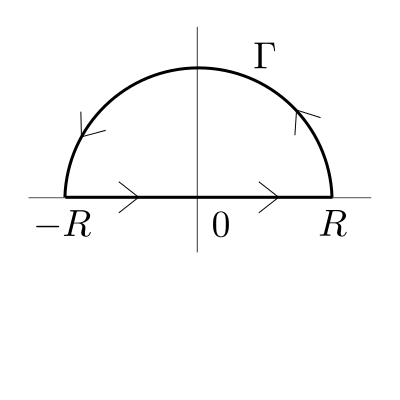
\includegraphics[width = 0.5\linewidth]{half-circle.png}
	\end{figure}

	As shown in the figure, let us denote the curvy part of the half-circle as $\Gamma$ and denote the whole half circle as $D$.

	Note that, $f(z) = \dfrac{e^{iz}}{(z^2 + 1)^2} = \dfrac{e^{iz}}{(z-i)^2}(z + i)^2$. Therefore, the function is analytic everywhere except at the poles $z = i$ and $z = (-i)$, where each of these poles are of order 2. However, only the pole $z = i$ would be inside the area enclosed by the half-circle $D$ for $R > 1$, hence, by an application of Residue Formula, it follows that;

	$$
	\int_D \dfrac{e^{iz}}{(z^2 + 1)^2}dz = 2\pi i \res_{z = i}(f)
	$$

	Notice that, as $z = i$ is a pole of order 2,

	\begin{align*}
		\res_{z = i}(f)
		& = \lim_{z \rightarrow i} \dfrac{d}{dz} \left[ (z-i)^2 f(z)\right]\\
		& = \lim_{z \rightarrow i} \dfrac{d}{dz} \dfrac{e^{iz}}{(z+i)^2}\\
		& = \lim_{z \rightarrow i} \dfrac{ ie^{iz} (z+i)^2 - 2e^{iz}(z+i) }{(z + i)^4}\\
		& = \dfrac{e^{-1}(-4)i - 2e^{-1}(2i)}{(2i)^4}\\
		& = -\dfrac{i}{2e}  
	\end{align*}

	Thus, 

	\begin{equation}
		\int_D \dfrac{e^{iz}}{(z^2 + 1)^2}dz = \dfrac{\pi}{e}	\qquad \forall R > 1 \label{eqn:6-1}
	\end{equation}

	Also, as the half-circle $D$ is union of two paths, namely the part of the real line $(-R, R)$ and $\Gamma$, we can rewrite \cref{eqn:6-1} as;

	\begin{equation}
		\int_{-R}^{R} \dfrac{e^{iz}}{(z^2 + 1)^2}dz + \int_\Gamma \dfrac{e^{iz}}{(z^2 + 1)^2}dz = \dfrac{\pi}{e} \qquad \forall R > 1	
		\label{eqn:6-2}
	\end{equation}

	Now, we shall show that, as $R \rightarrow \infty$, the second integral actually becomes arbitrarily small, thus the first integral will converge to $\pi/e$. To show that, consider a natural parametrization of the curve $\Gamma$, namely $\Gamma(\theta) = Re^{i\theta}$, where $\theta$ goes from $0$ to $\pi$. Then, $\Gamma'(\theta) = iRe^{i\theta}$. Hence,

	\begin{align*}
		\left\vert \int_\Gamma \dfrac{e^{iz}}{(z^2 + 1)^2} dz \right\vert 
		& = \left\vert \int_{0}^{\pi} \dfrac{e^{iRe^{i\theta}}}{\left( R^2e^{2i\theta} + 1 \right)^2} iR e^{i\theta} d\theta \right\vert \\
		& \leq \int_{0}^{\pi} \left\vert \dfrac{e^{iRe^{i\theta}}}{\left( R^2e^{2i\theta} + 1 \right)^2} iR e^{i\theta} \right\vert d\theta\\
		& \leq \int_{0}^{\pi} \vert iR e^{i\theta} \vert \dfrac{\vert e^{iRe^{i\theta}} \vert }{\vert (R^2 e^{2i\theta} + 1)^2 \vert} d\theta\\
		& = \int_{0}^{\pi} R \dfrac{\vert e^{iR(\cos \theta + i\sin \theta)} \vert }{\vert R^2 e^{2i\theta} + 1 \vert^2} d\theta \qquad \text{ since, } \vert e^{i\theta} \vert = 1 \\
		& \leq \dfrac{R}{(R^2 - 1)^2} \int_{0}^{\pi} \vert e^{iR\cos \theta} \vert \vert e^{-R\sin \theta} \vert d\theta\\
		& \qquad \qquad \text{since, by triangle inequality, } \vert R^2 e^{2i\theta} + 1\vert \geq \vert R^2 e^{2i\theta} \vert - \vert (-1)\vert = (R^2 - 1)\\
	\end{align*}

	Also note that, $R\cos\theta \in \R$, hence $\vert e^{iR\cos\theta} \vert = 1$, and since $0 < \theta < \pi$, it is clear that $R\sin\theta > 0$ and hence $\vert e^{-R\sin\theta} \vert < 1$. Therefore, we end up with;

	$$
	\left\vert \int_\Gamma \dfrac{e^{iz}}{(z^2 + 1)}dz  \right\vert \leq \dfrac{R\pi}{(R^2 - 1)^2} \rightarrow 0 \qquad \text{ as, } R \rightarrow \infty
	$$

	Thus, we have using \cref{eqn:6-2}, 

	\begin{equation}
		\lim_{R \rightarrow \infty} \int_{-R}^{R} \dfrac{e^{iz}}{(z^2 + 1)^2} dz = \dfrac{\pi}{e}
		\label{eqn:6-3}
	\end{equation}

	However, since $\int_{-R}^{R} \dfrac{e^{iz}}{(z^2 + 1)^2} dz = \int_{-R}^{R} \dfrac{\cos z}{(z^2 + 1)^2} dz + i \int_{-R}^{R} \dfrac{\sin z}{(z^2 + 1)^2} dz$, and both of the integrals are real valued, we must have,

	$$
	\int_{-\infty}^{\infty} \dfrac{\cos x}{(x^2 + 1)^2} dx = \lim_{R \rightarrow \infty} \Re\left[ \dfrac{e^{iz}}{(z^2 + 1)^2} dz \right] = \Re\left[ \lim_{R \rightarrow \infty} \dfrac{e^{iz}}{(z^2 + 1)^2} dz \right] = \Re\left[\dfrac{\pi}{e}\right] = \dfrac{\pi}{e}
	$$

	Finally, applying \cref{eqn:6-0}, we obtain the value of the desired integral,

	$$
	\int_{0}^{\infty} \dfrac{\cos x}{(x^2 + 1)^2} dx = \dfrac{\pi}{2e}
	$$














\end{answer}










\vspace*{1in}

\begin{center}
	{\Large\textit{Thank you}}
	\vspace*{0.25in}\\
	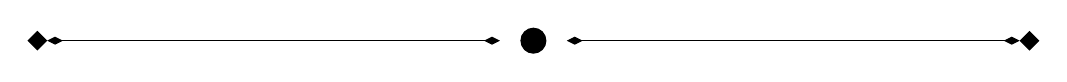
\begin{tikzpicture}[scale = 3]
		\node (a) at (0,0) {};
		\node (b) at (2,0) {};
		\draw[fill] (2.1, 0) circle (1.5pt);
		\node[draw, diamond, fill = black, scale = 0.5] at (0,0) {};
		\node (d) at (2.2,0) {};
		\node (e) at (4.2,0) {};
		\node[draw, diamond, fill = black, scale = 0.5] at (4.2,0) {};
		\draw [{Diamond}-{Diamond}] (a.east) -- (b.west);
		\draw [{Diamond}-{Diamond}] (d.east) -- (e.west);
	\end{tikzpicture}
\end{center}


\end{document}

